\documentclass[UTF8]{ctexart}
%\setmainfont{Noto Sans CJK SC}
\usepackage{xeCJK}
\setCJKmainfont[BoldFont=Noto Sans S Chinese Bold Bold]{Noto Sans S Chinese Regular}
\usepackage{amsmath}
\usepackage{geometry}
\geometry{a4paper, left=2cm, right=2cm,top=2cm,bottom=2cm}
\usepackage{pifont}
%\ding{172}=\textcircled{1}
\usepackage{booktabs}
\usepackage{hyperref}
\usepackage{mathrsfs}
\usepackage{graphicx}
\usepackage{wrapfig}
\usepackage{float}
\usepackage[perpage]{footmisc}
\newcommand{\firstsection}{\subsection}
\newcommand{\backdoc}{\normalsize}
\newcommand*{\dif}{\mathop{}\!\mathrm{d}}
\renewcommand{\thefootnote}{\ding{\numexpr171+\value{footnote}}}

\title{Part3 Interference}
\author{Xiao Liang}
\date{\today}

\begin{document}
	\maketitle
	\tableofcontents
	\numberwithin{equation}{section}
	%\CJKfontspec{Noto Sans Mono CJK SC}
	\CJKfontspec[BoldFont=Noto Sans S Chinese Bold Bold]{Noto Sans S Chinese Regular}
	\newpage
	简单地说,光学干涉就是两束或多束光波的相互作用,这种相互作用产生的总辐照度不等于各束光波的辐照度之和。
	
	干涉器件可以分为两种:分波阵面干涉和分振幅干涉。在前一种情况下,初级波阵面的各个不同部分或者直接用来做发射次级波的光源,或者和光学仪器联合作用产生次级波的虚光源,然后把这些次级波聚到一起产生干涉;在后一种情况下,初级波本身分成两份,走过了不同的光程之后,重新复合并发生干涉。
	
	\section{实际光波的干涉及实验方法}
	
	\subsection{一般情况}
	为了简单起见,我们考虑两个点光源$S_{1}$和$S_{2}$,它们在均匀媒介中发射同一频率的单色波。令两者间隔远大于波长,选择观察点$P$距离光源足够远,使得到了$P$点的两个波阵面都是平面。暂且我们只考虑如下的线偏振波:
	\begin{equation}
	\begin{aligned}
	\mathbf{E}_{1}(\mathbf{r}, t)&=\mathbf{E}_{01} \cos \left(\mathbf{k}_{1} \cdot \mathbf{r}-\omega t+\varepsilon_{1}\right)\\	
	\mathbf{E}_{2}(\mathbf{r}, t)&=\mathbf{E}_{02} \cos \left(\mathbf{k}_{2} \cdot \mathbf{r}-\omega t+\varepsilon_{2}\right)
	\end{aligned}
	\end{equation}
	
	由于辐照度和电场平方的平均值成正比,所以在现在的情况下,辐照度和以下值成正比:
	\begin{equation}
	\mathbf{E}^{2}=\left(\mathbf{E}_{1}+\mathbf{E}_{2}\right) \cdot\left(\mathbf{E}_{1}+\mathbf{E}_{2}\right)
	\end{equation}
	
	由此可得到:
	\begin{equation}
	I=I_{1}+I_{2}+I_{12}
	\end{equation}
	
	\noindent 其中,$I_{12}=2\left\langle\mathbf{E}_{1} \cdot \mathbf{E}_{2}\right\rangle$。这一项被称为\textbf{干扰项},在这里我们算出它的大小。
	
	考虑
	\begin{equation}
	\begin{aligned}
	\mathbf{E}_{1} \cdot \mathbf{E}_{2}=&\mathbf{E}_{01} \cdot \mathbf{E}_{02} \cos \left(\mathbf{k}_{1} \cdot \mathbf{r}-\omega t+\varepsilon_{1}\right)\\
	&\times \cos \left(\mathbf{k}_{2} \cdot \mathbf{r}-\omega t+\varepsilon_{2}\right)
	\end{aligned}\label{5.2}
	\end{equation}
	
	\noindent 同时我们知道某函数$f(t)$在时间间隔$T$内的时间平均值是
	\begin{equation}
	\langle f(t)\rangle=\frac{1}{T} \int_{t}^{t+T} f\left(t^{\prime}\right) \dif t^{\prime}
	\end{equation}
	
	\noindent 我们现在讨论的情况下$T \gg \tau$,这时积分前面的系数$\frac{1}{T}$有很重要的作用。方程\ref{5.2}可以化为:
	\begin{equation}
	\left\langle\mathbf{E}_{1} \cdot \mathbf{E}_{2}\right\rangle=\frac{1}{2} \mathbf{E}_{01} \cdot \mathbf{E}_{02} \cos \left(\mathbf{k}_{1} \cdot \mathbf{r}+\varepsilon_{1}-\mathbf{k}_{2} \cdot \mathbf{r}-\varepsilon_{2}\right)
	\end{equation}
	
	上式利用了$\left\langle\cos ^{2} \omega t\right\rangle=\frac{1}{2}$,$\left\langle\sin ^{2} \omega t\right\rangle=\frac{1}{2}$和$\langle\cos \omega t \sin \omega t\rangle=0$,于是干涉项为:
	\begin{equation}
	I_{12}=\mathbf{E}_{01} \cdot \mathbf{E}_{02} \cos \delta
	\end{equation}
	
	\noindent $\delta$是光程和初始相角差联合引起的相位差。
	
	考虑$E_{01}$和$E_{02}$平行的情况,在这种情况下,可以使用标量代替矢量。总的辐照度可以写做:
	\begin{equation}
	I=I_{1}+I_{2}+2 \sqrt{I_{1} I_{2}} \cos \delta\label{equ_I}
	\end{equation}
	
	当相位差是$2\pi$的整数倍时,得到辐照度的最大值,这时两个扰动被称为\textbf{同相}的,这种情况叫做\textbf{完全相长干涉}。当$0<\cos \delta<1$,两个波有相位差,$I_{1}+I_{2}<I<I_{\max }$,这个结果叫做\textbf{相长干涉}。同理,当$ 0>\cos \delta>-1 $时出现\textbf{相消干涉},而当$ \cos \delta =-1 $,得到辐射度的最小值,被称为\textbf{完全相消干涉}。
	
	方程\ref{equ_I}对于$S_{1}$和$S_{2}$发射的球面波同样成立,这时:
	\begin{equation}
\delta=k\left(r_{1}-r_{2}\right)+\left(\varepsilon_{1}-\varepsilon_{2}\right)
	\end{equation}
	
	辐射度极小值和极大值都位于一簇旋转双曲面中。

	\subsection{发生干涉的条件}
	1、两个光源之间的相位差$(\varepsilon_{1}-\varepsilon_{2})$必须随时间保持相当恒定,这样的光源也被称为\textbf{相干光源}。来自不同的发射源的互相交叠的两束光总是会产生干涉的,但是所得到的图样不能维持足够长的时间使得容易被观察到。

	2、两个光源的频率需要非常接近,以保证产生稳定的条纹。明显的频率差将引起与时间有关的迅速变化的相位差,它将使得在探测期间$I_{12}$的平均值为零。

	3、两个光源要有同一个方向的偏振分量。

	补充:当发生干涉的两个波的振幅相等或非常接近相等时,将有最清晰的图样。这时暗条纹和亮条纹的中心分别对应于完全相消干涉和完全相长干涉,从而形成最大的反衬度。

	对于光干涉的条件,菲涅尔-阿喇戈定律表述如下:

	1、两个正交的相干$\mathscr{P}$态不能发生干涉,即$I_{12}=0$,并且不产生条纹;

	2、两个平行的相干$\mathscr{P}$态以与自然光相同的方式发生干涉;

	3、自然光的两个正交$\mathscr{P}$态分量,即使把它转到一个方向,也不能发生干涉以产生能观察到的条纹图样。
	
	注意,在两个叠加光波的振动方向有一个夹角$ \alpha $时,在两个光波相平行的分量方向可以进行干涉,但垂直方向有一个分量会在观察屏上造成均匀照射,不利于干涉图样的观测。但一般夹角较小,这个分量可以忽略。
	
	\subsection{光波分离方法}
	将一个光波分离成两个相干光波,一般有两种方法。一种方法是让光波通过并排的两个小孔或利用反射和折射方法把光波的波前分割成为两个部分,这种方法称为\textbf{分波前法}。另一种方法是利用两个部分反射的表面通过振幅分割产生两个反射光波或两个透射光波,这种方法称为\textbf{分振幅法}。根据两种方法可以将产生干涉的装置分为两类:分波前装置和分振幅装置。前者只容许使用足够小的光学,而后者可以使用扩展光源,因而可获得强度较大的干涉效应,几乎所有实用的干涉仪都属于这部分。
	
	对于从一个光波分离处的两个光波,只有当它们通过的光程之差不是特别大时,才能发生干涉。这是由于光源辐射的光波本质上都是一段段有限的波列,如果它们到达相遇点时的光程差超过了波列长度便不能发生干涉,波列长度也被称为\textbf{相干长度}。
	
	\section{杨氏干涉实验}
	杨氏干涉实验时利用分波前法产生干涉的最著名的日子,通过对这一实验的分析,可以了解分波前法干涉的一些共同的特点。
	\begin{figure}[h]
		\centering
		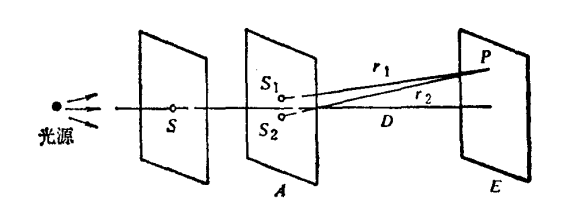
\includegraphics[width=12cm]{Yang.png}
		\caption{杨氏双缝干涉}
		\label{figure_Yang}
	\end{figure}

	实验装置如\ref{figure_Yang}所示。$ S $是一个受光源照明的小孔,从$ S $散出的光落在光屏$ A $的两个小孔$ S_{1} $和$ S_{2} $上,两者彼此相距很近,且到$ S $等距。从两个小孔再次散出的光波因为是同一个光波分割出来的,所以是相干光波。
	
	将$ S $以及$ S_{1} $和$ S_{2} $均视为单色点光源,并且因为等距,$ S_{1} $和$ S_{2} $是同相的。对屏幕上的某一点$ P $,两者发出的光在该点叠加产生的光强度,根据式\ref{equ_I}可以得知。若实验中两小孔大小相等,则有$ I=I_{1}=I_{2} $。因为两者同相,所以相位差$ \delta $只依赖于两者到$ P $点的光程差,设距离分别为$ r_{1},r_{2} $,则光程差为$ \Delta=n(r_{2}-r{1}) $,因而位相差为:
	\begin{equation}
		\delta = 2 \pi \frac{n(r_{2}-r_{1})}{\lambda}
	\end{equation}
	
\noindent  $ n $为介质的折射率,$ \lambda $为光波在真空中的波长。由此得$ P $点的光强度为:
\begin{equation}
I=2 I_{0}+2 I_{0} \cos \left[2 \pi \frac{\left(r_{2}-r_{1}\right)}{\lambda}\right]=4 I_{0} \cos ^{2}\left[\frac{\pi\left(r_{2}-r_{1}\right)}{\lambda}\right]
\end{equation}

\noindent 可见,$ P $点的光强强度决定于两光波的光程差,当屏幕上某些点满足条件
\begin{equation}
\Delta=r_{2}-r_{1}=m \lambda \quad(m=0, \pm 1, \pm 2 \cdots)
\end{equation}

\noindent 时,这些点的光强强度有极大值$ I=4I_{0} $。另一些点满足条件
\begin{equation}
\Delta=r_{2}-r_{1}=\left(m+\frac{1}{2}\right) \lambda \quad(m=0, \pm 1, \pm 2 \cdots)
\end{equation}

\noindent 时,这些点的光强强度有极小值$ I=0 $。其余的点的光强度在两者之间。

考虑杨氏双缝干涉的几何关系。
\begin{figure}[h]
	\centering
	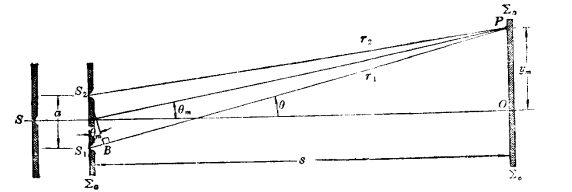
\includegraphics[width=12cm]{Yang1.png}
	\caption{杨氏双缝干涉几何图}
	\label{figure_Yang1}
\end{figure}

	在实际情况中,两个屏之间的距离要比两个狭缝之间的距离$ a $大得多,因而所有的条纹都很靠近中心$ O $。容易得到
	\begin{equation}
	\left(\overline{S_{1} B}\right)=\left(\overline{S_{1} P}\right)-\left(\overline{S_{2} P}\right)=r_{1}-r_{2}
	\end{equation}
	
	继续采用这个近似,光程差可以表现为:
	\begin{equation}
	r_{1}-r_{2}=a \theta
	\end{equation}
	
\noindent 注意到
	\begin{equation}
		\theta=\frac{y}{s}\label{equ_theta}
	\end{equation}
	
\noindent 所以
	\begin{equation}
		r_{1}-r_{2}=\frac{a}{s} y =m \lambda
	\end{equation}
	
\noindent 时发生\textbf{相长干涉}。由上式可以得到
\begin{equation}
	y_{m}=\frac{s}{a} m \lambda
\end{equation}

\noindent 如果我们把在$ O $处的极大值算作第零条条纹,上式就给出了屏上第$ m $条亮纹的位置,将上式代入式\ref{equ_theta}可以得到条纹的角位置:
\begin{equation}
	\theta_{m}=\frac{m \lambda}{a}
\end{equation}

	两个相邻极大值位置差为:
	\begin{equation}
	y_{m+1}-y_{m}=\frac{s}{a}(m+1) \lambda-\frac{s}{a} m \lambda
	\end{equation}
	
\noindent 或
\begin{equation}
	\Delta y=\frac{s}{a} \lambda
\end{equation}

	在屏幕上得到直线的干涉条纹是有条件的,条件就是$ d \gg D $,且在$ z $轴附近的小范围内观察。但是,由于在$ S_{1} $和$ S_{2} $发出的两相干光波的整个交叠区域内,均发生干涉现象,所以屏幕的位置实际上是可以任意安置的。这样,在屏幕任意放置的情况下,一般就得不到直线等条纹,此时要决定条纹的形状,必须首先求出两点光源干涉的那些等光程点的轨迹,因为干涉条纹是由光程差相同的各点联接而成的。可以证明,等光程差点在空间的轨迹是一个\textbf{回转双曲面}:
	\begin{equation}
	\frac{x^{2}}{\left(\frac{m \lambda}{2}\right)^{2}}-\frac{y^{2}+z^{2}}{\left(\frac{d}{2}\right)^{2}-\left(\frac{m \lambda}{2}\right)^{2}}=1
	\end{equation}
	
	\begin{figure}[h]
		\centering
		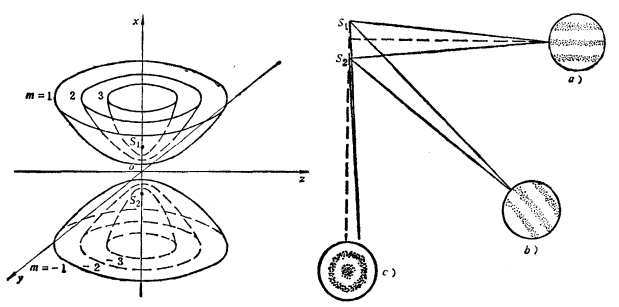
\includegraphics[width=12cm]{Interference1.png}
		\caption{等光程示意图和条纹形状随观察位置的变化}
		\label{figure_Interference1}
	\end{figure}

	在实际的杨氏干涉实验中,从小孔$ S_{1} $和$ S_{2} $散出的光波发散角不大,两光波的交叠区域只限于$ z $轴附近,所以实际上只能在图\ref{figure_Interference1}右a位置观察到干涉条纹,条纹是一些平行等距的直线。
	
	在相干光波交叠的区域内观察干涉条纹,除了用屏幕外,还可以用目镜放大或用照相机物镜照相。在干涉仪理论中,常常把观察屏幕、目镜焦平面或照相机底板所在的平面称为干涉场。
	
	有关其他干涉实验请直接翻看教材,此处不赘述。
	
	\section{条纹的可见度}
	干涉场中某一点$ P $附近条纹的清晰度用条纹的可见度(或称对比度)$ K $来量度,$ K $定义为
	\begin{equation}
	K=\frac{I_{M}-I_{m}}{I_{M}+I_{m}}\label{equ_K}
	\end{equation}
	
\noindent 式中$ I_{M} $和$ I_{m} $分别为$ P $点附近的强度极大值和极小值。两个强度相同的理想单色光源可以使得$ K=1 $,然而实际的干涉实验中这种情况不会发生发生。

	条纹的可见度与两相干光波的相对强度、光源大小和光源的单色性有关,下面根据控制变量法的思想进行讨论。
	
	\subsection{两相干光波强度不等的影响}
	当两光束强度不等时,根据式\ref{equ_I},干涉条纹强度极大值和极小值分别为$ \left(\sqrt{I_{1}}+\sqrt{I_{2}}\right)^{2} $和$\left(\sqrt{I_{1}}-\sqrt{I_{2}}\right)^{2}$,代入式\ref{equ_K}可得:
	\begin{equation}
		K=\frac{2 \sqrt{I_{1}} \sqrt{I_{2}}}{I_{1}+I_{2}}
	\end{equation}
	
\noindent 易见,当$ I_{1}=I_{2} $时,$ K=1 $;而两者相差越大,$ K $值越小。可以这样理解,若两相干光波的强度相差很大,则两相干光波所造成的强度实际上与较大强度光波单独产生的强度没有差别,也即是干涉场几乎一片均匀亮度,观察不出干涉条纹。
	
	还可以写成以下形式:
	\begin{equation}
		I=I_{t}(1+K \cos \delta)
	\end{equation}
	
\noindent 式中,$ I_{t}=I_{1}+I_{2} $。上式表明,干涉条纹的光强变化不仅与相位差有关,还跟两相干光波的振幅比有关$ \left(K=\frac{2 \left(\frac{A_{1}}{A_{2}}\right)}{1+\left(\frac{A_{1}}{A_{2}}\right)^{2}}\right) $。因此,若把干涉条纹记录下来,就等于把两相关光波振幅比和位相差这两方面的信息都记录下来了。

	\subsection{光源大小的影响}
	实际的光源不可能是理想的点光源,总有一定的大小,它包含着众多的点光源。 每一个点光源,在干涉装置中都形成一对相干的点光源,各对相干点光源在干涉场产生刻字的一组条纹,由于各点光源具有不同的位置,所以各组条纹相互之间将产生一定的位移。这样,整个干涉场的强度分布不可能是理想的形状——暗条纹的强度不再为零,条纹的可见度下降。当光源大到一定程度时,空间干涉性被破坏,因而观察不到干涉条纹。
	
	(1)\ 光源的临界宽度
	
	\begin{figure}[h]
		\centering
		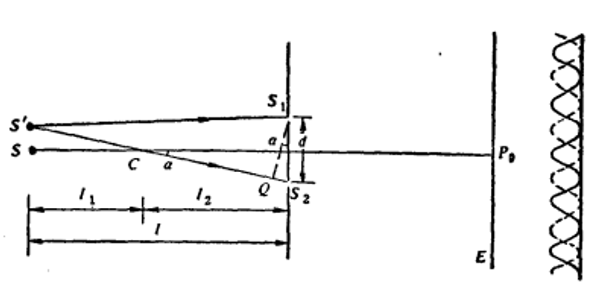
\includegraphics[width=10cm]{point_lights.png}
		\caption{两个点光源的杨氏实验}
		\label{figure_points}
	\end{figure}

	首先以杨氏实验为例,求出可见度下降到零时的临界宽度。假设光源只包含两个强度相等的发光点$ S $和$ S^{\prime} $,$ S $和$ S^{\prime} $在屏幕$ E $上各自产生一组条纹,两组条纹间距相等,但彼此有位移,若
	\begin{equation}
	S^{\prime} S_{2}-S^{\prime} S_{1}=\frac{1}{2} \lambda
	\end{equation}
	
\noindent 则$ S^{\prime} $在$ P_{0} $点产生极小强度,表明两个点光源产生的条纹彼此位移了半个条纹,如图\ref{figure_points}右面的曲线所示。图中实线表示$ S $产生的条纹,虚线表示$ S^{\prime} $产生的条纹。这两组条纹相加,使屏幕上处处强度相等,因此不可能观察到干涉条纹。
	
	现在,假定光源是以$ S $为中心的扩展光源$ S^{\prime}S^{\prime \prime} $
	
	\newpage
	\begin{figure}[ht]
		\centering
		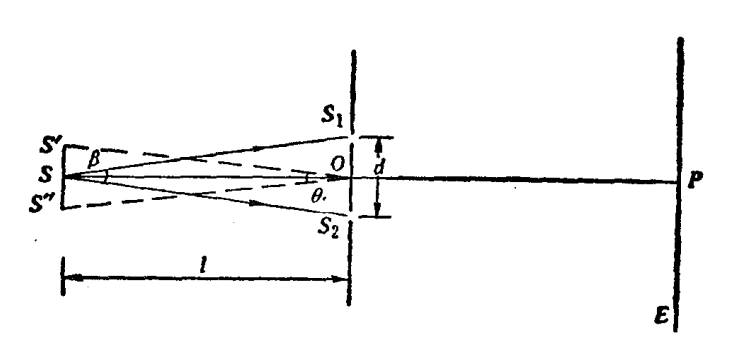
\includegraphics[width=12cm]{extern_lights.png}
		\caption{拓展光源的杨氏实验}
		\label{figure_extern_lights}
	\end{figure}

\noindent 则扩展光源所包含的每一个发光点都在屏幕上产生自己的一组条纹,整个扩展光源产生的条纹就是每一个点光源产生的条纹相加的结果。但是,当扩展光源的边缘点的光程差为半波长时,$ S $和$ S^{\prime} $产生的条纹时相互抵消的。设扩展光源的宽度$ S^{\prime}S^{\prime \prime}=b $,把扩展光源分为许多相距$ \frac{b}{2} $的点对,显然每一点对产生的条纹都相互抵消,因此整个扩展光源在屏幕上都不产生条纹。这时光源的宽度即为临界宽度。容易求出临界宽度的大小:
	\begin{equation}
S^{\prime} S_{2}-S^{\prime} S_{1} \approx S_{2} Q \approx \alpha d
	\end{equation}

\noindent 式中$ Q $是$ S^{\prime}S_{2} $与$ S_{1}S_{2} $的垂直平分线的交点$ C $到$ S_{1}S_{2} $所在的平面的距离,$ l_{1} $是$ SC $的距离。因此
\begin{equation}
l=l_{1}+l_{2} \approx\left(\frac{b}{2}+\frac{d}{2}\right) \frac{1}{\alpha}
\end{equation}

\noindent 或者
\begin{equation}
\alpha=\frac{b+d}{2 l}
\end{equation}

\noindent 所以
\begin{equation}
S^{\prime} S_{2}-S^{\prime} S_{1} \approx \alpha d \approx\left(\frac{b+d}{2 l}\right) d \approx \frac{b d}{2 l}
\end{equation}

\noindent 式中略去了d的平方项$ \frac{d^{2}}{2 l} $。这样,得到扩展光源不产生条纹的条件为:
\begin{equation}
	\frac{bd}{2 l}=\frac{\lambda}{2}
\end{equation}

\noindent 由此得出
\begin{equation}
	b=\frac{\lambda l}{d}
\end{equation}

\noindent 或
\begin{equation}
	b=\frac{\lambda}{\beta}\label{equ_b}
\end{equation}

\noindent 式中$ \beta=\frac{d}{l} $,称为干涉孔径,它是到达干涉场某一点的两支相干光从发光点$ S $射出的夹角。
	
	关系式\ref{equ_b}虽然是从杨氏干涉装置导出的,但可以证明它适用于前述的各种干涉装置,所以它是表示光源临界宽度和干涉孔径关系的一个普遍式子。
	
	(2)\ 条纹对比度随光源大小的变化
	
	光源大小在临界宽度范围内,干涉场上条纹的可见度随光源大小的的变化关系,可通过扩展光源所产生的条纹的强度分布得到。设每一个元光源的宽度为$ \dif x $,易见位于光源中点$ S $的远光源在干涉场某一点$ P $产生的光强度为:
	\begin{equation}
	\mathrm{d} I_{s}=2 I_{0} \mathrm{d} x\left(1+\cos \frac{2 \pi}{\lambda} \Delta\right)
	\end{equation}
	
\noindent 式中$ I_{0} \dif x $为宽度$ \dif x $的元光源的强度,$ \Delta $为元光源发出的两束相干光到达$ P $点的光程差。则对于距离$ S $点为$ x $的元光源,在$ P $点产生的光强度为:
	\begin{equation}
	\mathrm{d} I=2 I_{0} \mathrm{d} x\left[1+\cos \frac{2 \pi}{\lambda}(\Delta+x \beta)\right]
	\end{equation}
	
	因此,扩展光源在$ P $点产生的光强度为:
	\begin{equation}
		\begin{aligned}
		I=&\int_{-b / 2}^{b / 2} 2 I_{0}\left[1+\cos \frac{2 \pi}{\lambda}(\Delta+x \beta)\right] \dif x \\
		=&2 I_{0} b+2 I_{0} \frac{\lambda}{\pi \beta} \sin \frac{\pi b \beta}{\lambda} \cos \frac{2 \pi}{\lambda} \Delta
		\end{aligned}
	\end{equation}
	
	式中第一项与$ P $点的位置无关,表示干涉场的背景强度;第二项表示干涉场的光强度周期性地随$ \Delta $变化。由于第一项表示的背景强度会随着光源宽度的增大而不断增强,而第二项不超过$ I_{0} \frac{\lambda}{\pi \beta} $,所以随着光源宽度增大,条纹的可见性下降。
	
	容易得到(注意确定位置后,上式只有一个变量),干涉场的极大强度为:
	\begin{equation}
	I_{M}=2 I_{0} b+\left|\frac{2 I_{0} \lambda}{\pi \beta} \sin \frac{\pi b \beta}{\lambda}\right| 
	\end{equation}
	
\noindent 和极小强度:
\begin{equation}
I_{m}=2 I_{0} b-\left|\frac{2 I_{0} \lambda}{\pi \beta} \sin \frac{\pi b \beta}{\lambda}\right|
\end{equation}

\noindent 因此可得到条纹的可见度:
\begin{equation}
k=\frac{\lambda}{\pi b \beta} \sin \frac{\pi b \beta}{\lambda}
\end{equation}

	上式表明,随着光源宽度$ b $的增大,可见度通过一系列极大值与极小值而趋于零。第一个极小值对应于$ b \beta =\lambda $,这时的光源宽度即为临界宽度。

	一般认为,光源宽度不超过临界宽度的$ \frac{1}{4} $时,条纹的可见度仍时很好的,这时$ K \approx 0.9 $。这时的光源宽度称为许可宽度,为:
	\begin{equation}
		b_{p}=\frac{\lambda}{4 \beta}
	\end{equation}
	
	(3)\ 空间相干性
	
	从一个扩展光源照射出来的光,如果经过空间中两个点,且经过这两个点的光再次会合时能够发生干涉,则称通过空间的这两点的光具有空间相干性。显然,光的空间相干性与光源的大小紧密相关。从前面的讨论可知,当光源宽度
	\begin{equation}
		b=\frac{\lambda l}{d}\quad or \quad b=\frac{\lambda}{\beta}
	\end{equation}
	
\noindent 时,通过空间两点的光不发生干涉,也就是没有空间相干性。这个距离被称为\textbf{横向相干宽度},以$ d_{t} $表示,易见
\begin{equation}
	d_{t}= \frac{\lambda l}{b}
\end{equation}

\noindent 或用扩展光源对两点连线中点的张角表示:
\begin{equation}
	d_{t}=\frac{\lambda}{\theta}
\end{equation}

	理论证明,若光源时圆形的,上式还必须乘上一个因子1.22,即
	\begin{equation}
		d_{t}=\frac{1.22 \lambda}{\theta}
	\end{equation}
	
	而对于扩展光源为方形的情况,它照明的平面上的相干范围的面积(\textbf{相干面积})为:
	\begin{equation}
		A=d_{t}^{2}=\left(\frac{\lambda}{\theta}\right)
	\end{equation}
	
	\subsection{光源单色性的影响}
	干涉实验中实际使用的所谓单色光源,实际上包含一定的波长宽度$ \Delta \lambda $,这种情况自然会影响条纹的清晰度。各组条纹除了零级外,相互之间均为位移,各组条纹重叠的结果,使得条纹可见度下降。
	
	(1)\ 相干长度
	波长宽度为$ \Delta \lambda $的光源,能够产生干涉条纹的最大光程差,称为相干长度。假定在某一光程差下,波长为$ \lambda+\Delta \lambda $的$ m $级条纹和波长为$ \lambda $的$ m+1 $级条纹重合,那么相邻两极大值之间便充满了$ \Delta \lambda $范围内其他波长的极大值,因而该处没电强度相等,条纹的可见度为零。但此时光程差比较小的$ m $级以下的条纹尚能看见,由此可知相干长度:
	\begin{equation}
		\Delta_{max}=(m+1)\lambda=m(\lambda+\Delta \lambda)
	\end{equation}
	
\noindent 由此得到条纹对比度降为零时的干涉级别$ m=\frac{\lambda}{\Delta \lambda} $和相干长度$ \Delta_{max}=\frac{\lambda^{2}}{\Delta \lambda} $。

	上式表明,能够发生干涉的最大光程差与光源的光谱宽度成反比。而且容易知道,相干长度实际上就等于波列长度,用这两个概念来讨论干涉问题是完全等效的。
	
	(2)\ 条纹对比度于$ \Delta \lambda $和光程差得关系。
	
	光源的光谱宽度将使条纹对比度随着光程差$ \Delta  $的增大而下降。为简单起见,假设$ \Delta \lambda $内各个波长的光强度相等,或者以波数$ k=\frac{2 \pi}{\lambda} $表示,再$ \Delta k $宽度内不同波数的光谱成分的强度相等,根据式\ref{equ_I}和$ \delta =2 \pi \frac{r_{2}}{r_{1}} $可以得到元波数宽度$ \dif k $在干涉场产生的强度为:
	\begin{equation}
		\dif I=2 I_{0} \dif k (1+\cos k \Delta)
	\end{equation}
	
\noindent 式中,$ I_{0} $表示光强度的谱密度,即单位谱宽光波在干涉场的强度。在现在的假设条件下,它是常数。$ I_{0} \dif k $则是一束光在$ \dif k $元宽度内的强度。经过积分得到各个光谱成分产生的总强度为(设平均波数为$ k_{0} $):
\begin{equation}
	\begin{aligned}
		I=&\int_{k_{0}-\frac{\Delta k}{2}}^{k_{0}+\frac{\Delta k}{2}} 2 i_{0} (1+\cos k \delta)\\
		=&2 I_{0} \Delta k \left[1+\frac{\sin \left(\frac{\delta}{2}\right)}{\Delta k \frac{\delta}{2}} \cos(k_{0} \delta)\right]
	\end{aligned}
\end{equation}

\noindent 上式第一项是常数,表示干涉场的平均光强度;第二项随光程差$\delta$(在这部分为了和$ \Delta k $区别暂时使用$ \delta $,之后恢复正常) 大小变化,但变化的幅度越来越小。由上式可以得到条纹的对比度:
\begin{equation}
	K=\left|\frac{\sin \left(\Delta k \frac{\delta}{2}\right)}{\Delta k \frac{\delta}{2}}\right|
\end{equation}

	\begin{figure}[ht]
		\centering
		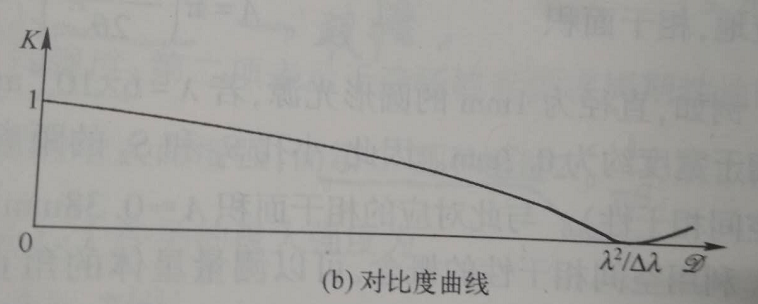
\includegraphics[width=12cm]{compare_lights.png}
		\caption{对比度曲线}
		\label{figure_compare_lights}
	\end{figure}

	在这里假定$ \Delta \lambda$内的光谱强度为等强度分布是不实际的,实际上应该是“类高斯分布”。如果知道光谱强度分布的具体函数形式,原则上可以把干涉场的强度分布和对比度求出来。可以证明,采用高斯型的分布函数,求出的对比度曲线和图\ref{figure_compare_lights}的曲线基本类似,最大光程差依旧可以用$ \Delta_{max}=\lambda^{2}/\Delta \lambda $表示。
	
	(3)\ 时间相干性
	
	光在一定光程差下能够发生干涉的事实表现了光波的时间相干性。光通过相干长度需要的时间即为时间相干。由同一光源在相干时间内不同时刻发出的光,经过不同的路径到达干涉场能够产生干涉,这种相干性便是时间相干性。由之前的结果可以得到:
	\begin{equation}
		\Delta_{max}= c \cdot \Delta t =\lambda^{2}/\Delta \lambda
	\end{equation}
	
\noindent 考虑到存在如下的关系(证明十分简单):
	\begin{equation}
		\frac{\Delta \lambda}{\lambda}=\frac{\Delta v}{v}
	\end{equation}

\noindent 联合上面两式可以得到:
	\begin{equation}
		\Delta t \cdot \Delta v=1
	\end{equation}
	
\noindent 经过简单变换便可以得到其中一个不确定关系,由此可以看出不确定关系就是由波动观点自然推导而出的。

	\section{平行平板产生的干涉}
	之前的讨论都是用分波前法产生的干涉,这类干涉现象需要宽度很小的光源,实用性不大。实际上,在应用干涉方法进行测量时,为了增加条纹的亮度,需要采用宽度较大的光源,这时就需要使用分振幅干涉。对于平板的分振幅干涉,就是\textbf{利用平板的两个表面对入射光的反射和透射,使入射光的振幅分解为两个部分,这两个部分光波相遇产生干涉}。
	
	平板可以理解为受两个表面限制而成的一层透明物质,最常见的情形就是玻璃平板和夹于两块玻璃板间的空气薄层。当平板的两个表面是平面而且相互平行时,称为\textbf{平行平板}或\textbf{平行平面板}。两个平面相互成一楔角时,称为\textbf{楔形平板}。先考虑前一种平板。
	
	\subsection{条纹的定域}
	如果是点光源,假设其单色性足够好,那么不管观察点$ P $位于干涉场$ E $中的任何位置,都必然有从点光源$ S $出发的两束光到达:一支光从平半的上表面反射到P,另一支经上表面折射、下表面反射,再由上表面折射到$ P $。这些干涉条纹表现为同心圆环条纹,并且不论$ E $距离平板距离多远,都能够在上面看到清晰的干涉条纹。这种由点光源照明所产生的条纹称为\textbf{非定域干涉}。但如果光源$ S $为扩展光源时,由光源上不同点出发的到达$ P $点的两支相干光的光程差则不相同,或者说,光源上不同点在$ P $附近产生的条纹之间有唯一,因此$ P $点附近条纹的对比度将降低。当$ S $的横向宽度超过一定限度的时候,对比度下降为零,干涉条纹消失。然而,在平行平板的情况下,总可以找到一个平面,使得即使使用扩展光源,其对比度也不会降低,这个平面被称为\textbf{定域面},其上观察到的条纹被称为\textbf{定域条纹}。
	
	干涉条纹的定于问题,实际上是一个空间相干性问题,对于下图左边的情形,如果光源的横向宽度为$ b $,$ P $点对应的干涉孔径为$ \beta $,则根据空间相干性理论,要在$ P $点观察到干涉条纹必须满足条件:
	\begin{equation}
		b \beta < \lambda
	\end{equation}
	
	当$ b=b_{c}=\frac{\lambda}{\beta} $时,$ P $点处的条纹消失。但是,在$ \beta=0 $所确定的区域却可以观察到清晰的条纹,因此该处对应的光源的临界宽度为无穷大。可以用作图法定出定域面,对于平行平板,可以证明定域面在无穷远处。但如果用望远镜进行观察(如下图右),则可以知道,望远镜的焦平面$ F $就是定域面。由于两支反射光是由同一支入射光经平面两表面的反射和透射,进行振幅分解分出来的,所以可以知道,在无穷远处或者望远镜焦平面上观察到的干涉是一种分振幅干涉。
	\begin{figure}[ht]
		\centering
		\begin{minipage}[t]{0.48 \textwidth}
			\centering
			\includegraphics[width=6cm]{point_light.png}
			\caption{点光源照明平行平板产生的干涉}
		\end{minipage}
		\begin{minipage}[t]{0.48 \textwidth}
			\centering
			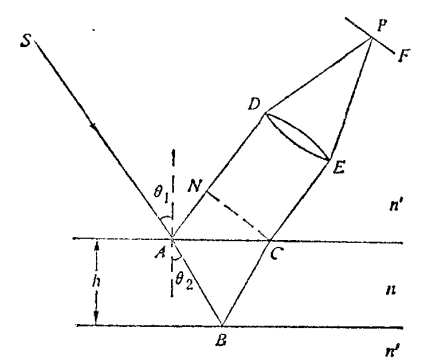
\includegraphics[width=6cm]{extern_light.png}
			\caption{平行平板的分振幅干涉}
			\label{figure_parallel}
		\end{minipage}
	\end{figure}

	\subsection{等倾条纹}
	考虑图\ref{figure_parallel}的情形,两束反射光的光程差为:
	\begin{equation}
		\Delta =n (AB-BC)-n^{\prime} AN
	\end{equation}
	
\noindent 式中,$ n $和$ n^{\prime} $分别是平板折射率和周围介质的折射率,$ N $是从$ C $点向$ AD $所引起的垂线的垂足。自$ N $点和自$ C $点到物镜焦平面上$ P $点的光程相等。

	设平面平板的厚度为$ h $,入射光在平板上表面的入射角和折射角分别为$ \theta_{1} $和$ \theta_{2} $,可以得到:
	\begin{equation}
		\Delta= 2 h \sqrt{n^{2}-n^{\prime 2} \sin^{2} \theta_{1}} \label{equ_Delta}
	\end{equation}
	
	如果平板的折射率与周围介质的折射率不同,则需要考虑光在平板表面反射时产生的\textbf{“半波损失”}所引起的附加光程差$ \lambda/2 $。(“半波损失”是波从波疏介质向波密介质的反射过程中所产生的相位差相差$ \pi $的情况)。
	
	在知道了两支反射光的强度和光程差之后,就可以写出焦平面上的强度表达式
	\begin{equation}
		I=I_{1}+I_{2}+2 \sqrt{I_{1} I_{2}} \cos \frac{2 \pi \Delta}{\lambda}
	\end{equation}

\noindent 可见,随着焦平面上不同位置对应的$ \Delta $的变化,我们将得到一组亮暗条纹。亮暗条纹分别对应着$ \Delta= m \lambda $和$ \Delta = (m+\frac{1}{2}) \lambda $,其中,$ m=1,2,3,... $。

	如果平行平板是绝对均匀的,折射率$ n $和厚度$ t $均为常数,那么光程差只决定于入射光在平板上的入射角$ \theta_{1} $(或折射角$ \theta_{2} $)。因此,\textbf{凡入射角相同的光束就形成同一干涉条纹}。由于这样的原因,通常把这种干涉条纹称为\textbf{等倾条纹}。
	
	由于等倾条纹完全对应于光束的入射角,由此可知在扩展光源照明情况下,等倾条纹仅出现在特定的观察平面上,所以条纹是定域条纹。
	
	\subsection{圆形定域条纹}
	等倾条纹的形状与观察望远镜的方位有关。一般情况下等倾条纹的形状为椭圆形,只有当望远镜光轴与平板法线平行的时候,才会使一组同心圆条纹,圆形位于望远镜的焦点,这通常称为\textbf{海定格条纹}。由上一节可知,在焦平面上的等倾圆条纹半径只和倾角有关,光源的每一点都给出彼此准确重合的等倾圆条纹,这使得光源的扩大增加增加干涉条纹的强度,并不会影响到条纹的对比度。
	
	下面导出等倾圆条纹的角半径和间距的表达式。设条纹中心的干涉级为$ m_{0} $,则有:
	\begin{equation}
		2 n h+\frac{\lambda}{2} =m_{0} \lambda
	\end{equation}
	
\noindent $m_{0}$不一定是整数(即中心未必是最亮点),它还可以写做:
\begin{equation}
	m_{0}=m_{1}+q
\end{equation}

\noindent 从中心向外计算,第$ N $个条纹的干涉级显然是$ \left[m_{1}-(N-1)\right] $,因而该条纹的角半径$ \theta_{1N} $(条纹半径对物镜$ L $中心的张角)可由下式求出:
\begin{equation}
	2 h \sqrt{n^{2}-n^{\prime 2} \sin ^{2} \theta_{1 N}} \pm \frac{\lambda}{2}=\left[m_{1}-(N-1)\right] \lambda
\end{equation}

\noindent 两式相减可以得到:
\begin{equation}
	2 n h\left(1-\cos \theta_{2 N}\right)=( N-1+q) \lambda
\end{equation}

\noindent 一般情况下,$ \theta_{1 N} $和$ \theta_{2N} $都很小,考虑一阶近似,可以由上式得到:
\begin{equation}
	\theta_{ 1 N} \approx \frac{1}{n^{\prime}} \sqrt{\frac{n \lambda}{h}} \sqrt{N-1+q}
\end{equation}

\noindent 上式表明,条纹的半径与$ \sqrt{\frac{1}{h}} $成比例,因此用较厚的平板产生的圆条纹要比较薄的平板产生的圆条纹半径要小一些(在同是第$ N $个亮条纹相比)。根据这个关系,可以利用等倾圆条纹来检验平板的质量。检验时,可直接用眼睛观察。当平板水平移动时(或眼睛水平移动时),平板的另一部分面积发生作用,如果平板是理想的平行平板,各处的折射率和厚度均相同,则在平板移动时人眼看到的圆条纹的直径保持不变。如果平板不均匀,则当平板移往较薄的部分时,条纹直径增大;平板移往较厚的部分时,条纹直径缩小,这样就可以达到检验平板光学厚度$ (nh) $均匀性的目的。

	利用式$ \ref{equ_Delta} $,还可以导出等倾条纹的角间距$ \Delta \theta_{1} $(相邻两条纹对物镜中心的张角)的表达式。两边求微分且令$ \dif m=1 $可得:
	\begin{equation}
		\Delta \theta_{2} = - \frac{\lambda}{2 n h \sin \theta_{2}}
	\end{equation}
	
\noindent 式中,负号仅表示随着$ \theta_{2} $的增大,$ \Delta \theta_{2} $单调减小,可以只考虑其绝对值。对折射定律取微分,并且考虑近似,能够得到$ \Delta \theta_{2} \approx \frac{n^{\prime} \Delta \theta_{1}}{n} $。于是,得到条纹的角间距为:
	\begin{equation}
	\Delta \theta_{1} \approx-\frac{n \lambda}{2 n^{\prime 2} \theta_{1} h}
	\end{equation}
	
\noindent 可见,$ \Delta \theta_{1} $与$ \theta_{1} $成反比,这表示靠近中心的条纹较疏,离中心越远,条纹越密。另外,平板越厚,条纹也越密。

	\subsection{透射光条纹}
	在透射光干涉的情况下,由光源$ S $到达望远镜焦平面上某一点$ P $的两支光,一支是直接从平板两表面透过的光,另一支是经过平板两次内反射后透过的光,如下图所示。
	
\noindent 当平板两边的介质相同时,这两支光的光程差为:
\begin{equation}
	\Delta = 2n h \cos \theta_{2}
\end{equation}

\noindent 这时没有反射相位变为引起的附加光程差,因为在平板两表面的内反射是在相同条件下发生的。然而,当平板两边介质不同且平板反射率介于两边介质的折射率之间时,一样会发生“半波损失”,这个时候就需要加上附加光程差$ \frac{\lambda}{2} $了。不难看出,对于同一入射角的光束来说,两支透射光的光程差和两支反射光的光程差正好相差$ \frac{\lambda}{2} $,位相差相差$ \pi $。所以,透射光的等倾条纹图样和反射光的等倾条纹图样是\textbf{互补}的。

	透射光条纹还有一个特点,当平板平面的反射率很低时,接近正入射时的反射率约为0.04,这时发生干涉的两支透射光强度相差很大,透射光等倾条纹的对比度因而很低。而对于反射光条纹,发生干涉的两支反射光相差很小,所以反射光条纹的对比度要好得多。由于这样的原因,在平板反射率很低的情况下,通常利用的是反射光条纹。
	\newpage
	
		\begin{figure}[htbp]
		\centering
		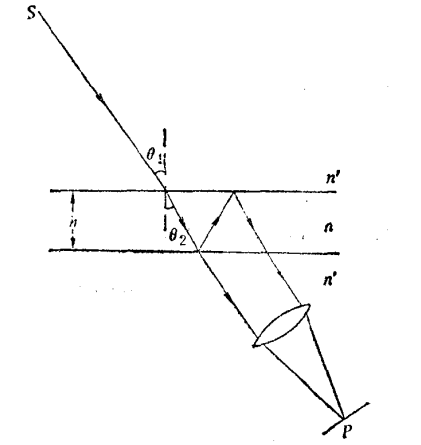
\includegraphics[width=12cm]{traver_light.png}
		\caption{透射光等倾条纹的形成}
		\label{figure_traver}
	\end{figure}

	\section{楔形平板产生的干涉}
	如同平行平板,楔形平板也可以产生非定域干涉和定域干涉。
	\begin{figure}[H]
		\centering
		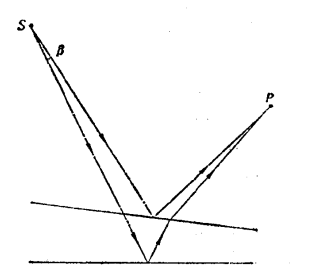
\includegraphics[width=6cm]{xie_point_light.png}
		\caption{点光源照明楔形平板产生的干涉}
		\label{figure_xie_point}
	\end{figure}

	图\ref{figure_xie_point}所示便是在点光源照明下的楔形平板。这时,对于平板外的任一点$ P $都有两支发自光源并经平板两表面反射的干涉光到达,所以这种条纹是\textbf{非定域}的。同样,当光源是扩展光源时,干涉条纹是定域的。
	
	\subsection{定域面的位置及定域深度}
	利用作图法令$ \beta=0 $可以得到楔形平板的干涉定域面,一般是个空间曲面。
	\begin{figure}[htbp]
		\centering
		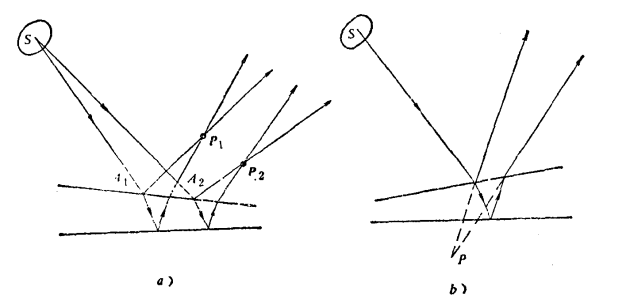
\includegraphics[width=12cm]{xie_extern_light.png}
		\caption{用扩展光源时楔形平面所产生条纹的定域面}
		\label{figure_xie_extern}
	\end{figure}

\noindent 由图\ref{figure_xie_extern}可见,当光源与楔形板的棱边各在一方时,定域面在楔形板的上方;而当光源与楔形板棱边在同一方时,定域面在楔形板的下方。楔形平板两表面的楔角越小,定域面离平板越远,平板称为平行平板时,定域面过渡到无穷远处。

	在楔形平板两表面的楔角\textbf{不是太小}或者\textbf{研究对象是厚度变化的薄膜}的情况,如果厚度足够小,定域面实际上很接近楔形平板或薄膜的表面。因此,观察薄板产生的定域干涉条纹,通常把眼睛、放大镜或显微镜调节在薄板的表面。
	
	对于一定宽度的扩展光源,在定域面周围一定的距离里还是能够看到条纹。如果把使用扩展光源时能够看到干涉条纹的区域称为定域区域的话,那干涉定域时具有一定深度地。显然,定域深度的大小与光源宽度成反比。
	
	\subsection{楔形平板产生的等厚条纹}
	设光源中心点$ S $发出的一支入射光在经平板两表面反射后,所分离出的两支光相交于定域面某一点$ P $,两支光在$ P $点的干涉效应由两支光的光程差决定:
	\begin{equation}
		\Delta=n(AB+BC)-n^{\prime}(AP-CP)
	\end{equation}
	
\noindent 式中,$ n $是楔形平板的折射率,$ n^{\prime} $是周围介质的折射率。光程差的精确值一般很难计算,但是在实用的干涉系统中,板的厚度一般都很小,并且楔角不太大,因此可近似地用平行平板地计算公式来代替,即:
\begin{equation}
	\Delta=2n h \cos \theta_{2}
\end{equation}

\noindent 	式中,$ h $是楔形平板在$ B $点的厚度,$ \theta_{2} $是入射光在$ A $的折射点。考虑到光束在平板上表面和下表面之一反射时的半波损失引起的附加光程差,上式应该改写为:
\begin{equation}
	\Delta=2n h \cos \theta_{2}+\frac{\lambda}{2}
\end{equation}

\noindent 如果所研究的楔形平板的折射率是均匀的,且光束的入射角为常数,譬如光源距平板较远或观察干涉条纹用的仪器的孔径很小,以至在整个视场内光束的入射角可视为常数,则有上式可知,两支反射光在相交点$ P $的光程差只依赖于反射光反射所处平板的厚度$ h $,因此干涉条纹与平板上厚度相同点的轨迹(等厚线)相对应,这种条纹称为\textbf{等厚条纹}。(严格上说,等厚条纹与平板上光学厚度$ nh $相同点的轨迹对应。当平板很薄时,定域区域实际上延伸到薄板的表面,因此我们注视薄板的表面就会看到这种沿薄板等厚分布的干涉条纹。

\begin{wrapfigure}{l}{6cm}
	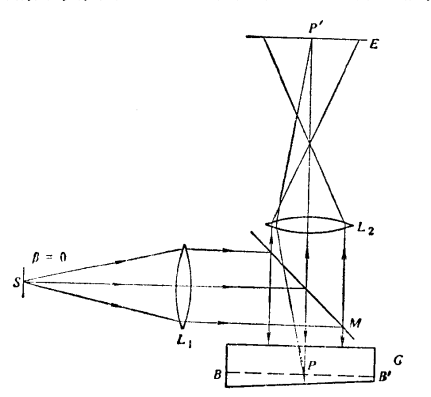
\includegraphics[width=6cm]{xie_practical.png}
	\caption{观察板上等厚条纹的一种使用系统}
	\label{figure_xie_practical}
\end{wrapfigure}

	对于厚度较大的平板,如果光束倾斜入射,定域面离平板较远,干涉定域深度也较小,一般不容易进行条纹干涉。在这种情况下可以使用图\ref{figure_xie_practical}所示的实用系统。这一系统对研究薄板条纹也十分有利。图中$ S $为扩展光源,位于准直透镜$ L_{1} $的前焦面上,$ S $发出的光束经透镜$ L_{1} $准直后射向玻璃片$ M $,再从玻璃片反射垂直投射到楔形平板$ G $上。入射光束在楔形平板上表面的反射光有原路回去,透过玻璃片$ M $后射向观察显微镜$ L_{2} $;在楔形平板下表面的反射光透过平板上表面和玻璃片射向$ L_{2} $。按照确定定域面的作图法,可知定域面在楔形平板内部的$ BB^{\prime} $位置。如果平板不是太厚,且平板两表面的楔角不是太大时,定域面非常接近平板下表面,这样如果调节显微镜$ L_{2} $对准平板下表面,就可在显微镜像平面$ E $上观察到楔形平板产生的等厚条纹。
	
	对于定域面上一点$ P $,扩展光源在该点产生的干涉效应,可由光源中心点在该点的光程差(垂直照明情况下)
	\begin{equation}
		\Delta=2nh+\frac{\lambda}{2}
	\end{equation}
	
\noindent 决定。当光程差满足条件
\begin{equation}
	\Delta= 2nh +\frac{\lambda}{2} =m \lambda \quad m=0,1,2,...
\end{equation}

\noindent 时,$ P $点是强度极大点。同理,当$ \Delta=\left(m+\frac{1}{2}\right) $时,$ P $点时强度极小点。对于楔形平板,厚度相同点的轨迹时平行于楔棱的直线。所以,楔形平板所产生的等厚条纹时一些平行于楔棱的等距直线。不同平板的等厚条纹如下:
\begin{figure}[ht]
	\centering
	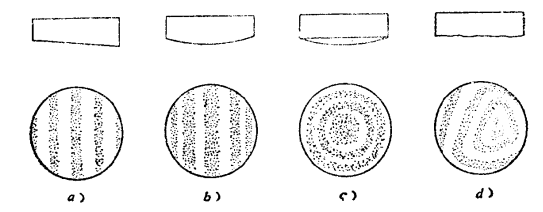
\includegraphics[width=12cm]{xie_denghou.png}
	\caption{几种不同形状的平板的等厚条纹}
	\label{figure_xie_denghou}
\end{figure}

	显然,不管哪一种情况,相邻两亮条纹或暗条纹对应的光程差之差都为$ \lambda $,所以从一个条纹过渡到相邻的一个条纹,平板的厚度改变$ \frac{\lambda}{2 n} $。考虑楔板的楔角,可以得到楔形平板相邻两亮条纹或暗条纹之间的距离,即\textbf{条纹间距}为:
	\begin{equation}
		e=\frac{\lambda}{2 n \alpha}\label{equ_e}
	\end{equation}
	
\noindent 式中,$ \alpha $是楔板的楔角,这里设它很小。对于两玻璃平板夹成的空气楔层,$ n=1 $。由之前的讨论可知,\textbf{条纹的间距与楔角成反比}。这一结论不仅适用于楔形平板,也适用于其他形状表面的等厚条纹。

	由式\ref{equ_e}可知,条纹间距与光波波长有关,波长较长的光形成的条纹间距较大,反之亦然。因此,使用白光光源时,除光程差等于零的零级条纹为白色外,零级附近的条纹将带有颜色。当空气层厚度比较大时(3—4个波长),由于白光的时间相干性的影响,条纹消失。根据白光条纹的两个特点:(1)\ 在零光程差处为白光;(2)\ 条纹颜色标志一定光程差的大小——可以利用帮光条纹来确定零程差位置和按颜色来估计光程差的大小。
	
	\subsection{等厚条纹的应用}
	\begin{wrapfigure}{l}{6cm}
		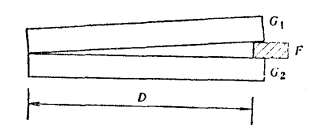
\includegraphics[width=6cm]{xie_rule.png}
		\caption{两块平板夹成的楔形空气层}
		\label{figure_xie_rule}
	\end{wrapfigure}
	
	等厚条纹可以用来进行测量,这里仅以测量薄片的厚度为例。如图\ref{figure_xie_rule},两块平板在$ G_{1} $和$ G_{2} $之间,一端完全贴合,另一端垫有厚度为$ h $的薄片$ F $,因而在两块平行平板之间形成一个楔形空气薄层,薄层一段的厚度为零,另一端的厚度为$ h $。将此用在图\ref{figure_xie_rule}中,将可看到空气层所产生的等距直线条纹。若已知光波波长为$ \lambda $,测量出楔形空气层的长度为$ D $,所产生条纹的间距为$ e $,那么空气层的最大厚度,即薄片$ F $的厚度可由下式计算:
	\begin{equation}
		h=\frac{D}{e} \cdot \frac{\lambda}{2}
	\end{equation}
	
	\section{用牛顿环测量透镜的曲率半径}
	\begin{wrapfigure}{l}{6cm}
		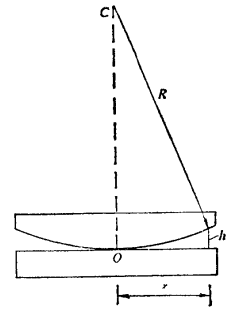
\includegraphics[width=6cm]{Newton_circle.png}
		\caption{牛顿环的形成}
		\label{figure_Newton_circle}
	\end{wrapfigure}

	在一块平面玻璃上,放置一个曲率半径$ R $很大的平凸透镜(图\ref{figure_Newton_circle}),在透镜的凸表面和玻璃板的平面之间便形成一个厚度由零逐渐增大的空气薄层。当以单色光垂直照射时,在空气层上形成一组以接触点$ O $为中心的中央疏、边缘密的圆形条纹,称为\textbf{牛顿环}\footnote{牛顿环条纹形状与等倾圆条纹相同,但牛顿环内圈的干涉级小,外圈的干涉级大,跟等倾圆条纹正好相反}。
	
	\subsection{测量原理}
	设测量出由中心向外计算的第$ N $个暗环的半径为$ r $,由图\ref{figure_Newton_circle}可见:
	\begin{equation}
		r^{2}=R^{2}-(R-h)^{2}=2 R h-h^{2}
	\end{equation}
	
\noindent 式中,$ R $是透镜凸表面的曲率半径,$ h $是该暗环对应的空气层厚度,由于$ R $较$ h $大得多,上式中可略去$ h^{2} $项,因此:
\begin{equation}
	h=\frac{r^{2}}{2 R}
\end{equation}

\noindent 将此式代入第$ N $个\textbf{暗环}满足的光程差条件
\begin{equation}
	2 h+\frac{\lambda}{2}=(2 m+1) \frac{\lambda}{2}
\end{equation}

\noindent 得到:
\begin{equation}
R=\frac{r^{2}}{m \lambda}
\end{equation}

\noindent 由上式可见,若以读数显微镜准确测出第$ N $个暗环的半径$ r $,已知所用单色光波长,即可计算出透镜的曲率半径。

	当透镜的曲率半径很大时,透镜凸表面和玻璃板平面之间空气层的厚度很小,如采用白光光源,即可看到彩色的牛顿环条纹。在圆环中心,对所有波长来说,光程差都等于$\frac{\lambda}{2}$,所以中心斑点是黑色的。从中心向外,一般额能看到三四个彩色圆环,一般来说,他们的颜色次序一定。再往外,随着空气层厚度的增大,彩色条纹消失,看到的是均匀的白色照明。
	
	\section{平面平行板的多光束干涉}
	前面分析干涉时只考虑了两条光线(反射线或折射线),实际上由于光束在平板中不断地反射和透射,在平板表面的反射系数比较高时,必须考虑多光束参与干涉才不会带来很大的误差。
	
	\subsection{干涉场的强度公式}
	\begin{figure}[ht]
		\centering
		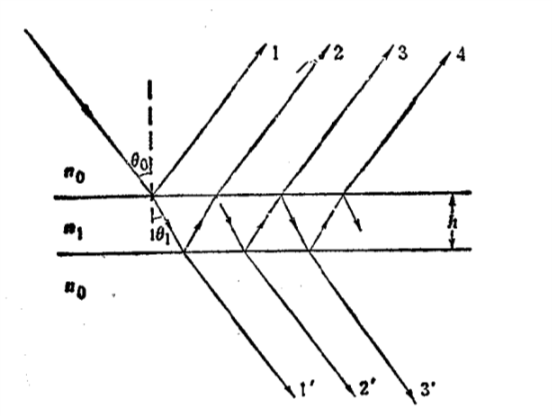
\includegraphics[width=12cm]{Interference_lights.png}
		\caption{光束在平行平板内的多次反射和透射}
		\label{figure_lights}
	\end{figure}

	现在考虑干涉场上任一点$ P $的光强度。容易知道,平行板的定域面在无穷远处,所以可以让光线通过透镜汇聚在焦平面上,因此平行板附近可视为平行光。由图\ref{figure_lights}可知,与$ P $点对应的多光束的出射角为$ \theta_{0} $,它们在平板内的入射角为$ \theta $,因而相继两束光(除去光束1,它的反射情况与后面不同,存在半波长的附加光程差)的光程差为:
	\begin{equation}
	\Delta=2 n h \cos \theta
	\end{equation}
	
\noindent 而相位差为
\begin{equation}
\delta=\frac{4 \pi}{\lambda} n h \cos \theta
\end{equation}

	在此之后需要考虑反射系数和透射系数(定义为振幅之比),从而得到一系列的光矢量的复振幅。在平板足够长,反射光束的数目很大的情况下,可以得到:
	\begin{equation}
	A^{(r)}=\left(r+\frac{t t^{\prime} r^{\prime} e^{i \delta}}{1-r^{\prime 2} e^{i \delta}}\right) A^{(i)}
	\end{equation}
	
\noindent 利用菲涅耳公式容易证明
\begin{equation}
	\begin{aligned}
		r&=-r^{\prime}\\
		t t^{\prime}&=1-r^{2}
	\end{aligned}
\end{equation}

\noindent 再考虑平板表面反射率$ R $和透射率$ T $(相关关系为:$ r^{2}=r^{\prime 2}\quad t t^{\prime}=1-R=T $)可以得到
\begin{equation}
A^{(r)}=\frac{\left(1-e^{i \delta}\right) \sqrt{R}}{1-R e^{i \delta}} A^{(i)}
\end{equation}

	由此得到反射光在$ P $点的光强度为
	\begin{equation}
	I^{(r)}=A^{(r)} \cdot A^{(r) *}=\frac{4 R \sin ^{2} \frac{\delta}{2}}{(1-R)^{2}+4 R \sin ^{2} \frac{\delta}{2}} I^{(i)}\label{equ_I_r}
	\end{equation}

	用同样的方法可以得到透射光在对应的$ P^{\prime} $点的强度:
	\begin{equation}
	I^{(t)}=A^{(t)} \cdot A^{(t) *}=\frac{T^{2}}{(1-R)^{2}+4 R \sin ^{2} \frac{\delta}{2}} I^{(i)}\label{equ_I_t}
	\end{equation}
	
	式\ref{equ_I_r}和式\ref{equ_I_t}即为所求的反射光干涉场和透射光干涉场的强度分布公式,通常也称为\textbf{爱里公式}。
	
	\subsection{干涉图样的特点}
	为讨论方便,引入参数
	\begin{equation}
		F=\frac{4 R}{(1-R)^{2}}\label{equ_F}
	\end{equation}
	
\noindent 这样式\ref{equ_I_r}和\ref{equ_I_t}可简化为
\begin{equation}
	\begin{aligned}
		\frac{I^{(r)}}{I^{(i)}}&=\frac{F \sin ^{2} \frac{\delta}{2}}{1+F \sin ^{2} \frac{\delta}{2}}\\
		\frac{I^{(t)}}{I^{(i)}}&=\frac{1}{1+F \sin ^{2} \frac{\delta}{2}}
	\end{aligned}
\end{equation}

\noindent 当忽略平板的吸收作用时,有
\begin{equation}
\frac{I^{(r)}}{I^{(i)}}+\frac{I^{(t)}}{I^{(i)}}=1
\end{equation}

\noindent 上式说明反射光和透射光的干涉图样互补。

	可以发现,干涉场的强度随$ R $和$ \delta $而变,在特定的$ R $的情况下,只随$ \delta $而变。因为$ \delta=\frac{4 \pi}{\lambda} n h \cos \theta $,所以光强度只和光束倾角有关,由此可知在这种情况下的多光束干涉在干涉场得到的是\textbf{等倾条纹}。当透镜的光轴垂直于平板时,得到的是同心圆环。条纹位置同只考虑两束光干涉时一模一样,反射光和透射光方向也是互补的。强度关系如下:
	\begin{equation}
		I_{M}^{(t)}=I^{(i)}\ and\ I_{m}^{(t)}=\frac{1}{1+F} I^{(i)}
	\end{equation}
	
	现在考虑条纹的强度分布随反射率$ R $的变化。当反射率$ R $很小时,由式\ref{equ_F}可知,$ F \ll 1 $,因此可以展开式\ref{equ_I_r}和\ref{equ_I_t},得到:
	\begin{equation}
	\begin{aligned}
	\frac{I^{(r)}}{I^{(i)}} \approx F \sin ^{2} \frac{\delta}{2}&=\frac{F}{2}(1-\cos \delta)\\
	\frac{I^{(r)}}{I^{(i)}} \approx 1-F \sin ^{2} \frac{\delta}{2}&=1-\frac{F}{2}(1-\cos \delta)
	\end{aligned}
	\end{equation}
	
	这正是两光束干涉条纹的强度分布,说明当反射率$ R $很小时可以只考虑两束光的干涉。当$ R $增大时,情况就有很大的不同。
	\begin{figure}[ht]
		\centering
		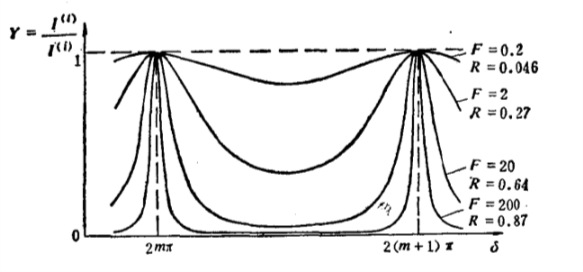
\includegraphics[width=12cm]{Interference_R.png}
		\caption{不同反射率下透射光条纹的强度分布曲线}
		\label{figure_R}
	\end{figure}

	\subsection{干涉条纹的锐度}
	干涉条纹的\textbf{锐度}定义为\textbf{条纹的相位差半宽度},指的是条纹中强度等于峰值强度一般的两点间的相位差距离,记为$ \Delta \delta $。对于第$ m $级条纹,两个半强度点对应的相位差为
	\begin{equation}
		\delta = 2m \pi \pm \frac{\Delta \delta}{2}
	\end{equation}
	
\noindent 考虑$ \Delta \delta $很小,可以得到条纹半宽度为
\begin{equation}
\Delta \delta=\frac{4}{\sqrt{F}}=\frac{2(1-R)}{\sqrt{R}}
\end{equation}

	定义\textbf{条纹的精细度}为相邻亮条纹间的距离($ 2 \pi $)和条纹半宽度之比
	\begin{equation}
S=\frac{2 \pi}{\Delta \delta}=\frac{\pi \sqrt{F}}{2}=\frac{\pi \sqrt{R}}{1-R}
	\end{equation}

\noindent 可以看出,当反射率$ R \rightarrow 1 $时,条纹变得愈来愈细,条纹的锐度愈好,一般情况下,多光束干涉更能达到这个要求,可以用来进行比较精密的测量,比如在光谱技术中测量光谱线的精细结构(塞曼效应)。

\section{法布里-珀罗干涉仪和陆末-盖尔克板}
这两种多光束干涉装置采用两种不同的方法来提高平板表面的反射率:前者是在平板的两表面镀一层金属膜或多层电介质反射膜;后者是适当选择光束的入射角,使光束在平板内的入射角略小于临界角。

\subsection{F-P干涉仪}
为了保证干涉仪两板之间保持严格平行,擦汗给你长在两板间放置一间隔圈制成的空心圆柱形间隔器,使两板间的距离不变,这种F-P干涉仪通常称为\textbf{法布里-珀罗标准具}。
\begin{figure}[H]
	\centering
	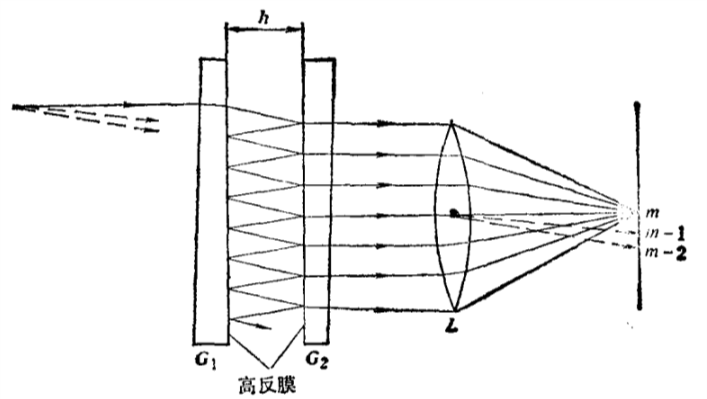
\includegraphics[width=12cm]{Interference_F-P.png}
	\caption{F-P干涉仪简图}
	\label{figure_F-P}
	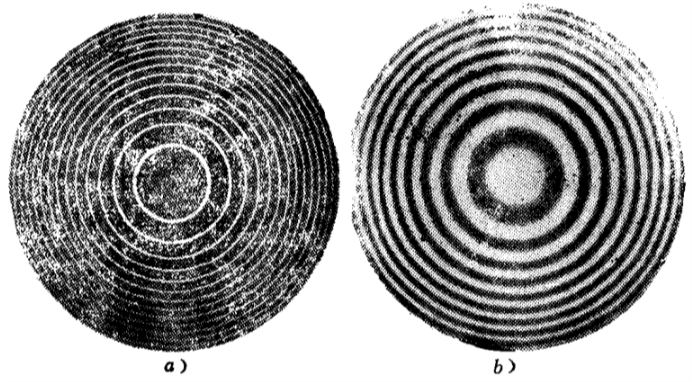
\includegraphics[width=12cm]{Interference_circle.png}
	\caption{多光束干涉条纹和两光束干涉条纹}
	\label{figure_circle}
\end{figure}

	干涉仪用扩展光源发出的发散光束照明,其中一支光的光路如图\ref{figure_F-P}所示。图\ref{figure_circle}左是该干涉仪在产生的同心圆条纹,可以看出,比起双光束干涉要精细得多。条纹的干涉级会很高,所以只适宜于单色性很好的光源。

	应该指出, 干涉仪两板的内表面镀金属膜时, 光在它表面反射的情况是比较复杂的。 但是, 只要两个膜层是相同的,投射的光强关系依然成立。不过,此时$ R $应理解为在金属膜内表面的反射率, 而相继两光束的位相差
	\begin{equation}
	\delta=\frac{4 \pi}{\lambda} h \cos \theta+2 \phi \label{equ_delta_}
	\end{equation}
	
\noindent 式中$ \phi $是在金属膜内表面反射时的位相变化。 另外, 光通过金属膜时将会发生强烈的吸收,使得整个干涉图样的强度降低。 设金属膜的吸收率为$ A $(吸收光强度与入射光强度之比),应有
\begin{equation}
R+T+A=1
\end{equation}

\noindent 因此,可以得到透射光干涉图样的强度公式为
\begin{equation}
\frac{I^{(t)}}{I^{(i)}}=\left(1-\frac{A}{1-R}\right)^{2} \frac{1}{1+F \sin ^{2} \frac{\delta}{2}}
\end{equation}

\noindent  与前面的公式对比可以发现,金属膜的吸收使得透射光图样的峰值强度下降了,严重时只有入射光的几十分之一。

	间隔固定的法布里-珀罗干涉仪(标准具) 常用来测量波长相差非常小的两条光谱线的波长差, 即光谱学中所谓超精细结构。 用一般的光学仪器, 如棱镜和光栅光谱仪是不容易把这种结构分开的。 
	设有两种波长$ \lambda_{1} $和$ \lambda_{2} $的光波投射到干涉仪上,由于同级条纹的角半径稍有差别,因而将得到如下图所示的双重条纹。
	\begin{figure}[H]
		\centering
		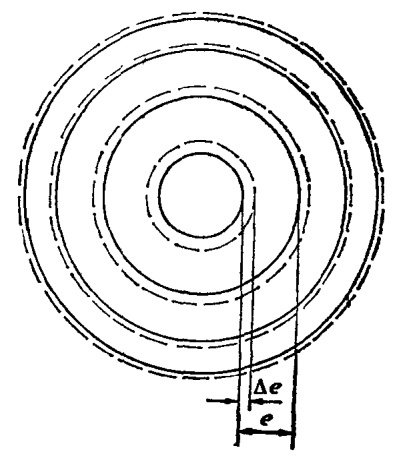
\includegraphics[width=10cm]{Interference_light.png}
		\caption{在法布里-珀罗标准具上显示出来的精细结构}
		\label{figure_light}
	\end{figure}

\noindent 对于靠近条纹中心的某一点,根据式\ref{equ_delta_}两组条纹的干涉差值是
\begin{equation}
\Delta m=m_{1}-m_{2}=\left(\frac{2 h}{\lambda_{1}}+\frac{\phi}{\pi}\right)-\left(\frac{2 h}{\lambda_{2}}+\frac{\phi}{\pi}\right)=\frac{2 h\left(\lambda_{2}-\lambda_{1}\right)}{\lambda_{1} \lambda_{2}}
\end{equation}

\noindent 同时,
\begin{equation}
	\Delta m =\frac{\Delta e}{e}
\end{equation}

\noindent 其中,$ \Delta e $是同级条纹的相对位移,$ e $是条纹间距,所以波长差为
\begin{equation}
	\Delta \lambda=\lambda_{2}-\lambda_{1}=\frac{\Delta e}{2 h e} \overline{\lambda}^{2}\label{equ_lambda}
\end{equation}

\noindent 其中$ h $是标准具间隔,平均波长则可以由分辨率本领较低的仪器预先测出。

	应用上述方法测量时,一般不应使两组条纹的相对位移$ \Delta e $大于条纹的间距$ e $,否则会发生不同级条纹的重叠现象。把$ \Delta e $恰好等于$ e $时对应的波长差称为\textbf{标准具常数或标准具的自由光谱范围},应用式\ref{equ_lambda}得到标准具的自由光谱范围
	\begin{equation}
	(\Delta \lambda)_{S.R}=\frac{\overline{\lambda}^{2}}{2 h}
	\end{equation}
	
\noindent 标准具的自由光谱范围即是标准具所能测量的最大波长差。

	除了自由光谱范围外,还有一个重要参数,即它能够分辨的最小波长差$ (\Delta \lambda)_{m} $,当波长差小于这个值时,两组条纹就不能被分开,它也被称为标准具的\textbf{分辨极限},而$ \frac{\overline{\lambda}}{(\Delta \lambda)_{m}} $称为\textbf{分辨本领}。在光谱仪其中,一般采用瑞利判据来判断两条等强度谱线是否被分开,即认为两个波长的亮条纹只有当它们的合强度曲线中央的极小值低于两边极大值的81\% 时才能被分辨开。
	
	由一对平面反射镜构成的腔体便是激光器的谐振腔。在谐振腔内沿轴线附近传播的光来回反射,通过激活介质不断地被放大,最后形成激光输出。由于激光的输出必须同时满足一定的频率条件和振荡阈值条件,所以激光输出实际上只有少数几种频率。在激光理论中,每一种输出频率称为一个\textbf{振荡纵模},每一种输出频率的频宽称为\textbf{单模线宽},而相邻两个纵模之见的间隔称为\textbf{纵模间隔},它们的表达式如下:
	
	(1) 纵模频率
	
	把谐振腔看作一个标准具的话,谐振腔的输出频率必须满足干涉亮纹的条件,在正入射的情况下,
	\begin{equation}
		2 n L = m \lambda \quad m=1,2,3,\cdots
	\end{equation}
	
\noindent 式中,$ n,L $分别为谐振腔内介质的折射率和腔体长度,$ m $是干涉级。由上式即可得到谐振腔的输出频率应该满足的条件:
\begin{equation}
	v= m \frac{c}{2 n L} \quad m=1,2,3,\cdots
\end{equation}

	(2) 纵模间隔
	由上式得:
	\begin{equation}
		\Delta v_{e} = v_{m} - v_{m-1} = \frac{c}{2 n L}
	\end{equation}
	
	(3) 单模线宽
	之前已经得到了多光束干涉条纹的位相差半宽度为
	\begin{equation}
		\Delta \delta = 2\frac{1-R}{\sqrt{R}}
	\end{equation}
	
\noindent 当光波包含许多波长时,与$ \Delta \delta $相应的波长差或谱线宽度可以这样求出:取$ \delta $因$ \lambda $变化的微分
\begin{equation}
\mathrm{d} \delta=-4 \pi n L \frac{\mathrm{d} \lambda}{\lambda^{2}}
\end{equation}

\noindent 或
\begin{equation}
|\Delta \delta|=4 \pi n L \frac{\Delta \lambda}{\lambda^{2}}
\end{equation}

\noindent 因为
\begin{equation}
\Delta \lambda=\frac{\lambda^{2}}{4 \pi n L}|\Delta \delta|=\frac{\lambda^{2} 1-R}{2 \pi n L \sqrt{R}}
\end{equation}

\noindent 因而频率表示的线宽为
\begin{equation}
\Delta \nu=\frac{c \Delta \lambda}{\lambda^{2}}=\frac{c}{2 \pi n L} \frac{1-R}{\sqrt{R}}
\end{equation}

\noindent 由上式可知,谐振腔的反射率越高,或腔长越长,线宽越小。

	\subsection{陆末-盖尔克板}
	陆末-盖尔克板是一块均匀的精确度要求很高的平行平面玻璃(或石英)板, 它之所以能够产生强度相近的多光束, 不是采用在平板的两表面涂反射膜层的方法, 而是采用前述的第二种方法, 即适当选择入射光束, 使光束在板内玻璃一空气界面的入射角略小于临界角,这样每次反射只有小部分光从板面透出, 而大部分光保留在板内。
	
	\begin{figure}[H]
		\centering
		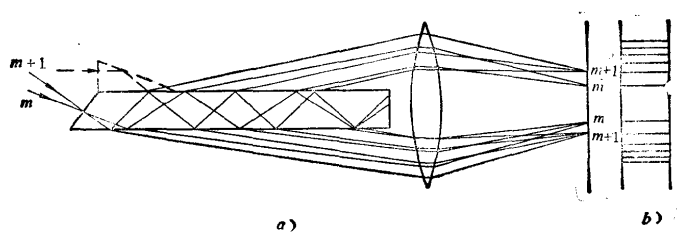
\includegraphics[width=12cm]{Interference_gaierke.png}
		\caption{陆末-盖尔克板产生的多光束干涉}
	\end{figure}
\end{document}
